%%% fs-seim-experiments - Experiments

\label {fs-experiments}

In order to estimate the performance, we implemented a prototype of the proposed approach. As a stream processing task, we apply the computation of inverted index for 1000 Wikipedia documents. The logical pipeline of this computation is shown in the figure ~\ref{inverted-index}. First map operation accepts Wikipedia documents and outputs pairs of words and corresponding positions. The next part of the pipeline accepts pairs of word and positions and computes updated index and the actual changelog. This stateful transformation is implemented in the form of groping and map operation with a cycle, as it was shown in the previous section. Regarding the physical deployment, the full logical graph is deployed on each computational unit or worker. Documents are randomly shuffled before the first map operation. Word positions are partitioned by word before grouping. The other links are implemented as simple chain calls.

\begin{figure}[htbp]
  \centering
  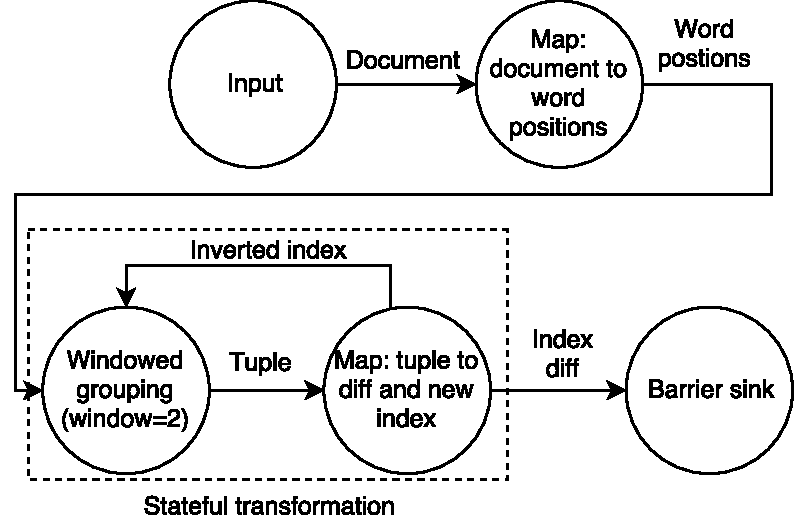
\includegraphics[width=0.48\textwidth]{pics/inverted-index}
  \caption{Logical pipeline for inverted index}
  \label {inverted-index}
\end{figure}

As a key metric in our experiment, we take the ratio of the all items arrived at the barrier to the valid items arrived at the barrier. This value clearly represents the overhead of our approach. The relation between the number of workers, the delay between input documents and the proposed ratio is shown in the figure ~\ref{experiment}. This figure demonstrates that the ratio of all items to the valid items is quite low even when the delay between documents is very short. Therefore, the experiment reveals that our approach is able to provide low network traffic overhead. 

\begin{figure}[htbp]
  \centering
  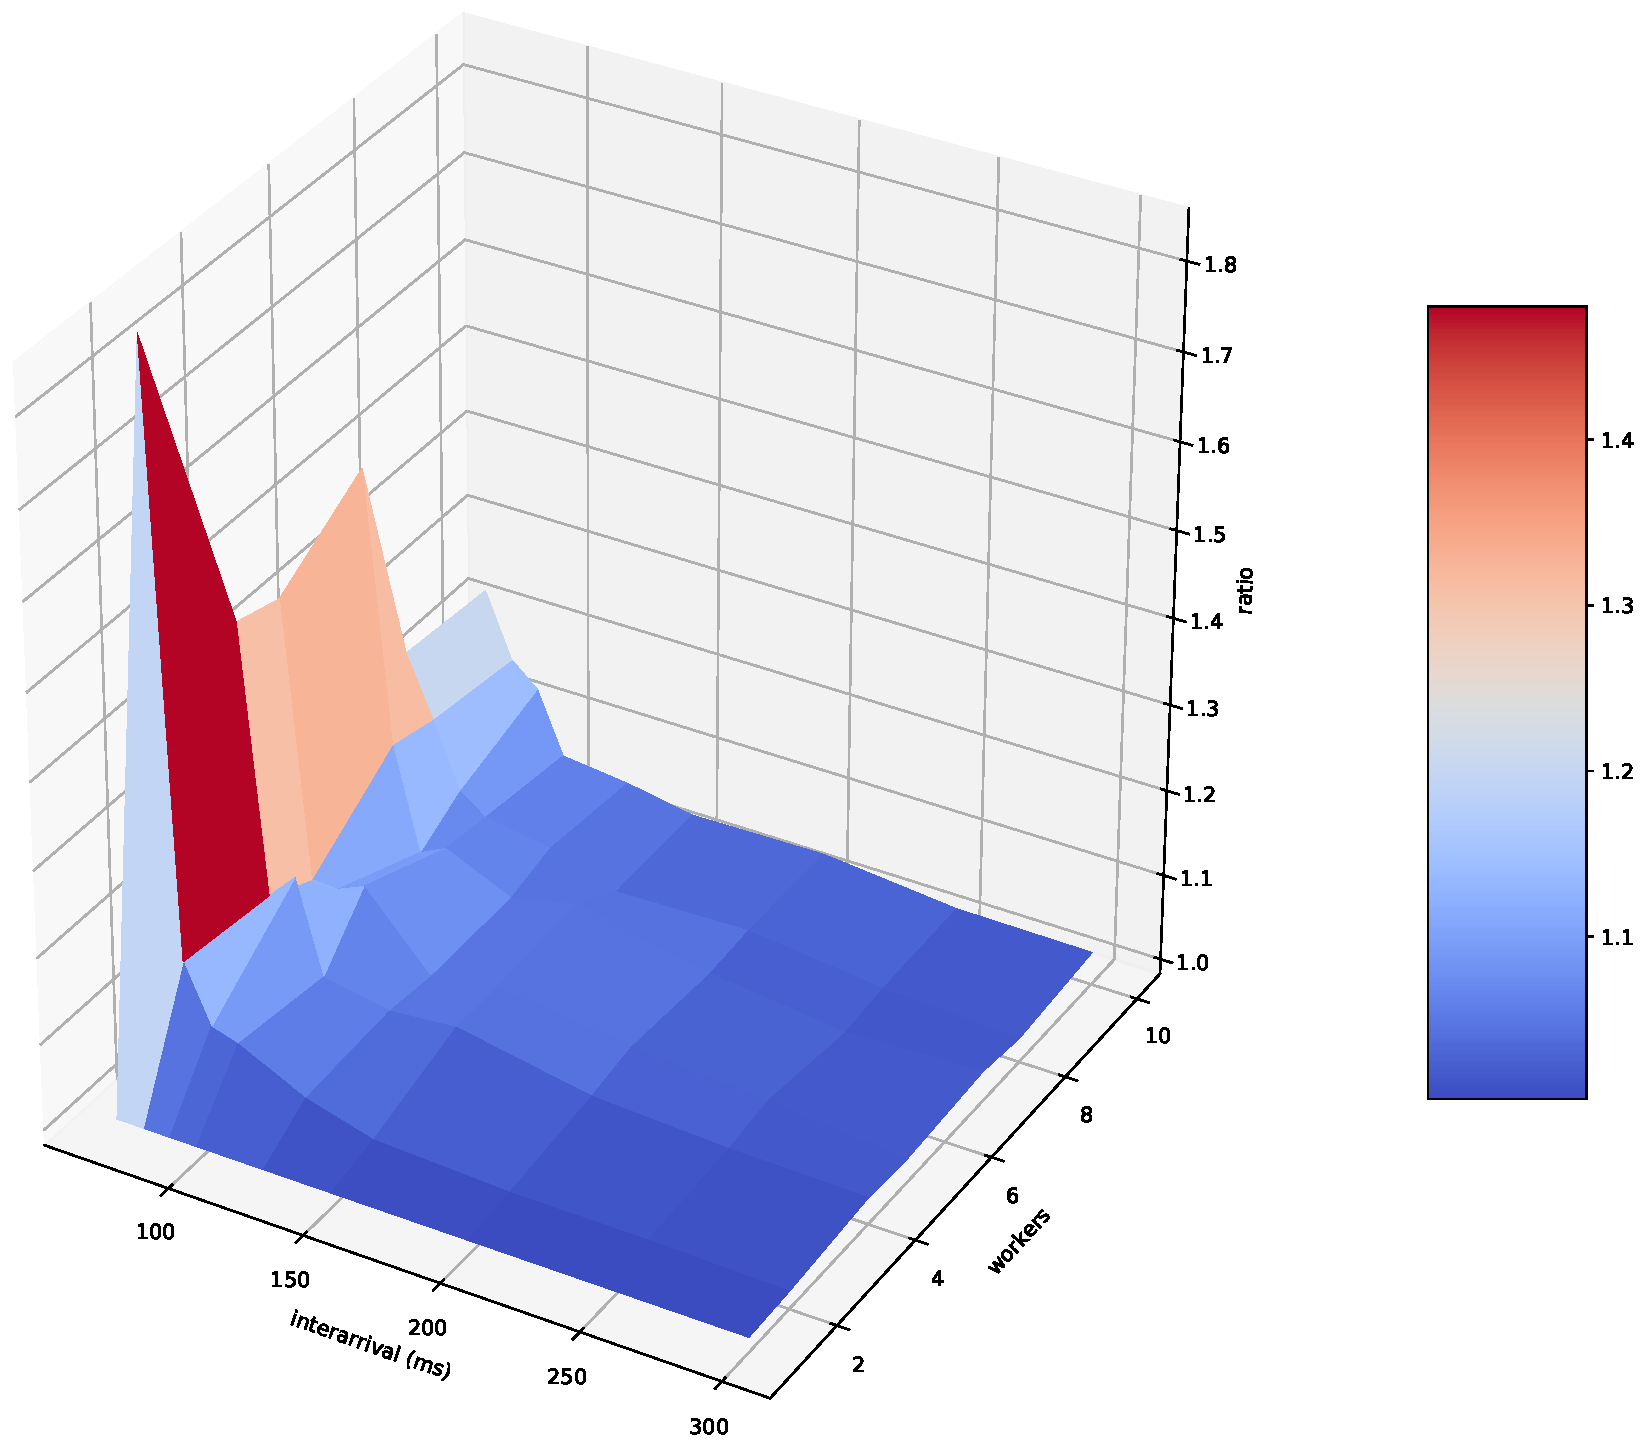
\includegraphics[width=0.48\textwidth]{pics/experiment}
  \caption{Experiment results}
  \label {experiment}
\end{figure}
